\documentclass[a4paper]{amsart}

\usepackage[utf8]{inputenc}

\usepackage{datetime2}
\usepackage{enumitem}
\usepackage{float}
\usepackage{graphicx} \graphicspath{{fig/}}
\usepackage{minted}



\begin{document}

\title[]{\lowercase{\texttt{rv32i}}\\---\\RISC-V RV32I emulator}
\author[]{\lowercase{selendym\\(selendym@tuta.io)}}
\date{\DTMnow}

\maketitle



\bigbreak
\section{Introduction}

\noindent
The subject of this project is the emulation of the RISC-V instruction-set architecture%
\footnote{https://riscv.org/specifications/}
(ISA), more precisely, the ``RV32I base integer instruction set'' variant, which is a 32-bit ISA.

The current implementation does what it should: it emulates RV32I and is able to run programs compiled with the GCC cross-compilation toolset for RISC-V bare-metal targets%
\footnote{https://aur.archlinux.org/packages/riscv64-unknown-elf-gcc/}.
As the implementation is ``bare-metal''%
\footnote{There is no support from the runtime environment, no operating system to handle system calls.},
the full C standard library cannot be used to write test programs.
However, to support \texttt{malloc}, the implementation does emulate handling of \texttt{sbrk} system calls, although very primitively.
Also, input-output (IO) is handled with custom \texttt{ecall} environment calls that are mapped to the standard input and output of the emulator.
The custom \texttt{ecall}s the test program uses are implemented with inline assembly, because C does not support executing arbitrary instructions directly.

The implementation provides a rudimentary command-line interface (CLI) for the emulator; this is described in more detail in subsection \ref{subsec:main}.



\bigbreak
\section{Structure}

\begin{figure}
    \centering
    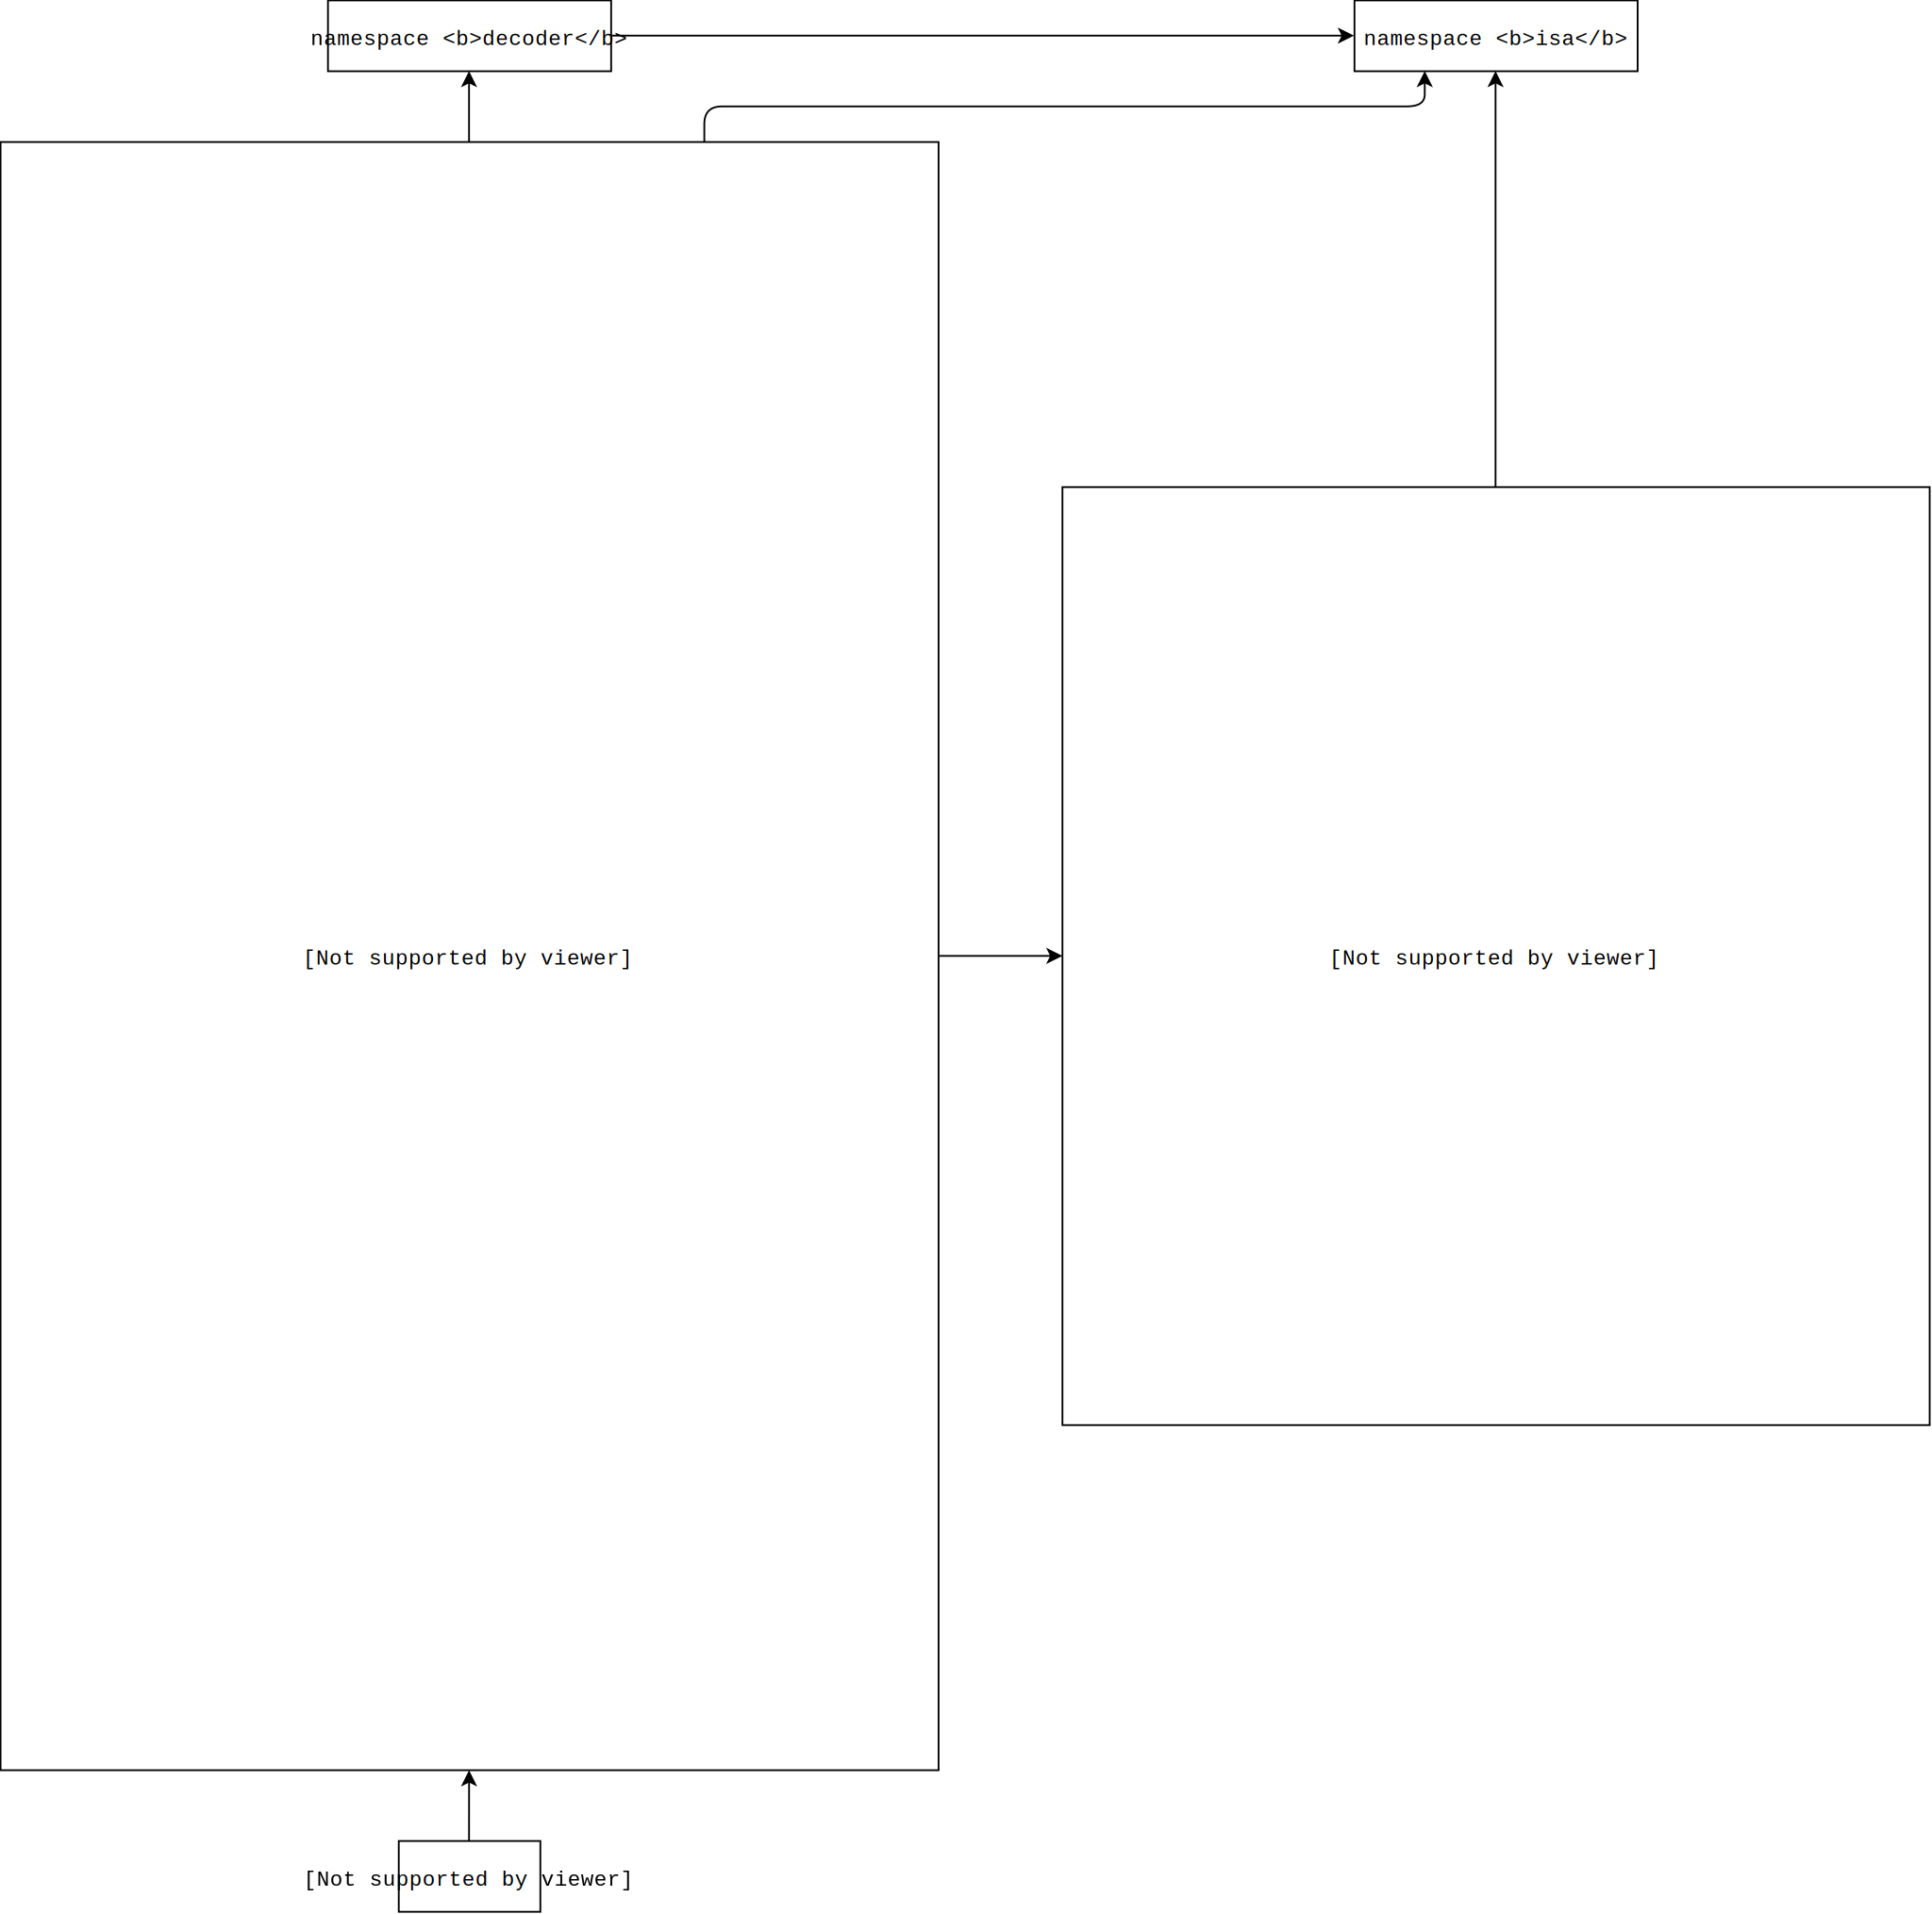
\includegraphics[width=1\columnwidth]{class_diag}
    \caption{Class diagram of the project.}
    \label{fig:class_diag}
\end{figure}

\noindent
A class diagram of the project is given in Figure \ref{fig:class_diag}.
Arrows represent dependencies and point from the requiring entity to the required one.


\medbreak
\subsection{Cpu}

\begin{listing}
    \begin{minted}[autogobble]{cpp}
        const reg_arr_t &get_reg_arr() const;
        const word_t &get_reg( reg_idx_t index ) const;
        const word_t &get_sp_reg() const;
        const word_t &get_pc_reg() const;
        void set_reg_arr( const reg_arr_t &reg_arr );
        void set_reg( reg_idx_t index, word_t value );
        void set_sp_reg( word_t value );
        void set_pc_reg( word_t value );
        void step();
    \end{minted}
    \caption{Public interface of class \texttt{Cpu}.}
    \label{list:cpu_public_interface}
\end{listing}

\noindent
Class \texttt{Cpu} (\texttt{src/cpu/cpu.\{h,c\}pp}) implements the main interface of the emulator proper.
Its public interface is given in Listing \ref{list:cpu_public_interface}.

\texttt{Cpu} implements the \texttt{get\_*} and \texttt{set\_*} member functions for getting and setting, and the \texttt{step} member function for advancing, the state of the emulation run.
Each invocation of \texttt{step} corresponds to the execution of the instruction (in emulated memory) pointed to by the current value of the \texttt{pc\_reg} data member.
With each step, \texttt{pc\_reg} is updated automatically; thus, to advance the emulation run, only \texttt{step} needs to be called.

Each invocation of \texttt{step} proceeds by executing in succession the functions \texttt{fetch}, \texttt{decode}, and \texttt{execute}.
\texttt{fetch} fetches the instruction to be executed from the (emulated) memory address corresponding to \texttt{pc\_reg}.
\texttt{decode} decodes the fetched instruction and returns a struct comprising the decoded fields.
\texttt{execute} executes the decoded instruction and changes the state of the emulation run accordingly.

\texttt{fetch} has a trivial implementation, and \texttt{decode} is described in detail in subsection \ref{subsec:decoder}.
The implementation of \texttt{execute} composes the body of \texttt{Cpu}.
Instructions are first divided into groups corresponding to their major opcodes.
These groups are then executed by their namesake functions; for example, \texttt{arith\_i} is responsible for executing the instructions belonging to the group ``immediate arithmetic''.


\medbreak
\subsection{Decoder}\label{subsec:decoder}

\begin{listing}
    \begin{minted}[autogobble]{cpp}
        instr_t decode( iword_t instr_word );
    \end{minted}
    \caption{``Public interface'' of namespace \texttt{decoder}.}
    \label{list:decoder_public_interface}
\end{listing}

\begin{listing}
    \begin{minted}[autogobble]{cpp}
        struct instr_t
        {
        // raw instruction word
            iword_t instr_word;
        // instruction-word bit fields
            opcode_e opcode;  // instr_word[ 6: 0]
            iword_t funct3;   // instr_word[14:12]
            iword_t funct7;   // instr_word[31:25]
            iword_t rd;       // instr_word[11: 7]
            iword_t rs1;      // instr_word[19:15]
            iword_t rs2;      // instr_word[24:20]
            word_t imm;  // variant; depends on opcode format type; sign-extended
        // decoded instruction and type
            opcode_type_e opcode_type;  // opcode format type
            mnem_e mnem;  // mnemonic; 'fully resolved opcode'; e.g., 'XOR'
        };  // END struct instr_t
    \end{minted}
    \caption{Struct \texttt{instr\_t}.}
    \label{list:instr_t}
\end{listing}

\noindent
Namespace \texttt{decoder} (\texttt{src/cpu/decoder.\{h,c\}pp}) implements the instruction decoder of the emulator.%
\footnote{\texttt{decoder} can be considered as a stateless class, comprising only (static) member functions.}
Its ``public interface'' is given in Listing \ref{list:decoder_public_interface}.

\texttt{decoder} implements the \texttt{decode} function for decoding a raw instruction word into an \texttt{instr\_t} struct (Listing \ref{list:instr_t}) comprising the decoded fields.
\texttt{decode} serves as the interface for decoding and performs some preliminary steps before calling more specific decoding functions.
As with \texttt{execute}, instructions are first divided into groups corresponding to their major opcodes.
These groups are then decoded by their namesake functions with \texttt{decode\_mnem\_} prepended; for example, \texttt{decode\_mnem\_arith\_i} is responsible for decoding the instructions belonging to the group ``immediate arithmetic''.
\texttt{decode\_imm} differs from the other functions by not belonging to any single group and is responsible for decoding immediate values for all groups.


\medbreak
\subsection{Memory}

\begin{listing}
    \begin{minted}[autogobble]{cpp}
        const uint8_t *get_mem_carr( addr_t addr = 0 ) const;
        uint8_t       *get_mem_carr_nc( addr_t addr = 0 );  // non-const
        const addr_t  &get_mem_size() const;
        uint8_t  lb( addr_t addr ) const;
        uint16_t lh( addr_t addr ) const;
        uint32_t lw( addr_t addr ) const;
        uint64_t ld( addr_t addr ) const;  // rv64i
        void sb( addr_t addr, uint8_t  word8 );
        void sh( addr_t addr, uint16_t word16 );
        void sw( addr_t addr, uint32_t word32 );
        void sd( addr_t addr, uint64_t word64 );  // rv64i
    \end{minted}
    \caption{Public interface of class \texttt{Memory}.}
    \label{list:memory_public_interface}
\end{listing}

\noindent
Class \texttt{Memory} (\texttt{src/cpu/memory.\{h,c\}pp}) implements the emulated memory system that \texttt{Cpu} uses.
Its public interface is given in Listing \ref{list:memory_public_interface}.

The \texttt{get\_mem\_size} member function returns the memory array size in (8-bit) bytes.
The \texttt{get\_mem\_carr} member function and its non-constant variant are used to provide direct access to the underlying raw memory array; these can be considered as a rudimentary form of direct memory access (DMA) and are used to provide a simple interface to IO functions.
The \texttt{l\{b,h,w,d\}} member functions allow addressed loads (reads) from a given memory location and return values of 8 (byte), 16 (half-word), 32 (word), and 64 (double-word) bits, respectively.
The \texttt{s\{b,h,w,d\}} member functions allow addressed stores (writes) to a given memory location of values of 8 (byte), 16 (half-word), 32 (word), and 64 (double-word) bits, respectively.

\texttt{Memory} implements the raw memory array using Linux system library call \texttt{mmap} to memory-map a file, serving as the memory image, onto the emulated memory address space.
The semantics of \texttt{mmap} allow any modifications made by the emulation run to transparently and automatically be mirrored in the memory image file, which can then be examined during or after the run to help in troubleshooting possible problems.


\medbreak
\subsection{ISA}

\begin{listing}
    \begin{minted}[autogobble]{cpp}
        using std::uint8_t,  std::int8_t;
        using std::uint16_t, std::int16_t;
        using std::uint32_t, std::int32_t;
        using std::uint64_t, std::int64_t;
        constexpr unsigned iword_length = 32;  // instruction bit width
        using iword_t = uint32_t;  // instruction word type
        using siword_t = int32_t;  // instruction word type; signed
        constexpr unsigned word_length = 32;  // register bit width
        using word_t = uint32_t;  // register word type
        using sword_t = int32_t;  // register word type; signed
        constexpr unsigned addr_length = word_length;  // memory address bit width
        using addr_t = word_t;  // memory address type
        constexpr unsigned reg_count = 32;  // register count
        constexpr word_t reg_0_value = 0;  // register-0 fixed value
        using reg_arr_t = std::array< word_t, reg_count >;
        using reg_idx_t = reg_arr_t::size_type;
        constexpr auto iword_mask = util::bit_mask< iword_t, iword_length >;
        constexpr auto iword_extract = util::bit_extract< iword_t, iword_length >;
        constexpr auto word_mask = util::bit_mask< word_t, word_length >;
        constexpr auto word_extract = util::bit_extract< word_t, word_length >;
        constexpr auto addr_mask = word_mask;
        constexpr auto addr_extract = word_extract;
        namespace reg_idx_ns;
        enum class opcode_type_e;
        enum class opcode_e;
        enum class mnem_e;
        struct instr_t;
    \end{minted}
    \caption{Contents of namespace \texttt{isa}.}
    \label{list:isa_contents}
\end{listing}

\noindent
Namespace \texttt{isa} (\texttt{src/cpu/isa.hpp}) implements the shared type definitions of the emulator.
Its contents are given in Listing \ref{list:isa_contents}.


\medbreak
\subsection{Main}
\noindent
Function \texttt{main} (\texttt{src/cpu/main.cpp}) implements a simple CLI for the emulator.


\medbreak
\subsection{Test}
\noindent
Function \texttt{main} (\texttt{src/test/test.c}) implements a test program for the emulator to run.



\bigbreak
\section{Instructions for building and usage}

\medbreak
\subsection{Main}\label{subsec:main}
\noindent
The CLI for the emulator, \texttt{main}, is built by invoking \texttt{make [all]} (the brackets signify optionality) in the \texttt{src/cpu} directory.
After a successful compilation, the \texttt{main} executable is located at \texttt{src/test/main}.
Note that a GCC version supporting \texttt{-std=c++17} is required.

Usage: \texttt{./main [<step\_count>] [<pc>] [<sp>]}

If \texttt{step\_count} is not given, the largest possible value, $-1$, is used (with unsigned arithmetic, this will wrap around).
Note that unless required, \texttt{pc} and \texttt{sp} should not be set explicitly; these correspond to the initial program counter (pc), which should point to the address of \texttt{\_start}, and the initial stack pointer (sp), which by default points to just past the end of the memory image.


\medbreak
\subsection{Test}
\noindent
The test program for the emulator, \texttt{test}, is built by invoking \texttt{make [all]} in the \texttt{src/test} directory.
After a successful compilation, two memory images, \texttt{mem.img.clean} and \texttt{mem.img} are created (the latter is simply a copy of the former).
Note that this step is optional, as a precompiled \texttt{mem.img.clean} is provided; otherwise, a GCC version supporting RISC-V bare-metal cross-compilation is required.

After an emulation run, the memory image file, \texttt{mem.img}, has most likely been modified by the run.
If desired, the image can be restored to a clean state by invoking \texttt{make reset-mem} in the \texttt{src/test} directory; this will also create the image if it does not exist.



\bigbreak
\section{Testing}

\noindent
Testing of the emulator proper was mostly realized by having the emulator run a test program compiled for the implemented ISA, RV32I, using GCC as a cross-compiler.
As the amount of differing instructions in RV32I is about 50 in total, a slightly more extensive test program should be able to cover these many times over.
In case bugs are present, it is very likely that the test program will not run correctly, if at all.
The lack of any unit tests was mostly due to lack of time and also of need in this particular case --- the coverage of the test program might not be 100\%, but it is likely reasonably close to this.

The test program is written mostly in C, with start-files and some utilities written in the RV32I subset of RISC-V assembly language.
As the target for compilation is bare-metal, custom start-files are required to set up and tear down the emulated environment to allow correct program execution.
Namely, the \texttt{\_start} and \texttt{\_exit} functions set up and tear down the emulation, respectively, and print diagnostic messages along the way to ease troubleshooting.

Due to the way the memory system is implemented, examining the contents of the emulated memory during or after an emulation run is made easy.
There are two files for the memory image, \texttt{mem.img.clean} and \texttt{mem.img}.
The former is the untouched, ``clean'', image, while the latter is the actually used memory image and may have changes made by the emulator.
The made changes are permanent, so if a ``clean'' emulation run is required, invoking \texttt{make reset-mem} in the test directory allows resetting the used memory image to the clean state.
To see the changes made in the memory image without great pains, a tool with hex diff capability is recommended%
\footnote{One such tool is \texttt{binwalk}, called with \texttt{binwalk --hexdump --red mem.img.clean mem.img}.}.

\end{document}
